\documentclass[handout]{beamer}
%\usepackage{beamerarticle}
\usepackage{tikz}
\usetikzlibrary{arrows,shapes}

\author{S.Poss}
\title{CHEP2012}
\subtitle{Review}

\mode<presentation>
{
  \usetheme{Singapore}
   \setbeamertemplate{navigation symbols}{}
   \setbeamertemplate{footline}[frame number] 
}

\AtBeginSection[]
{
\begin{frame}<beamer>
\frametitle{Outline}
\tableofcontents[currentsection,currentsubsection]
\end{frame}
}


\begin{document}
\begin{frame}
\begin{columns}[c]
\column{6cm}
\titlepage
\column{6cm}
\begin{center}
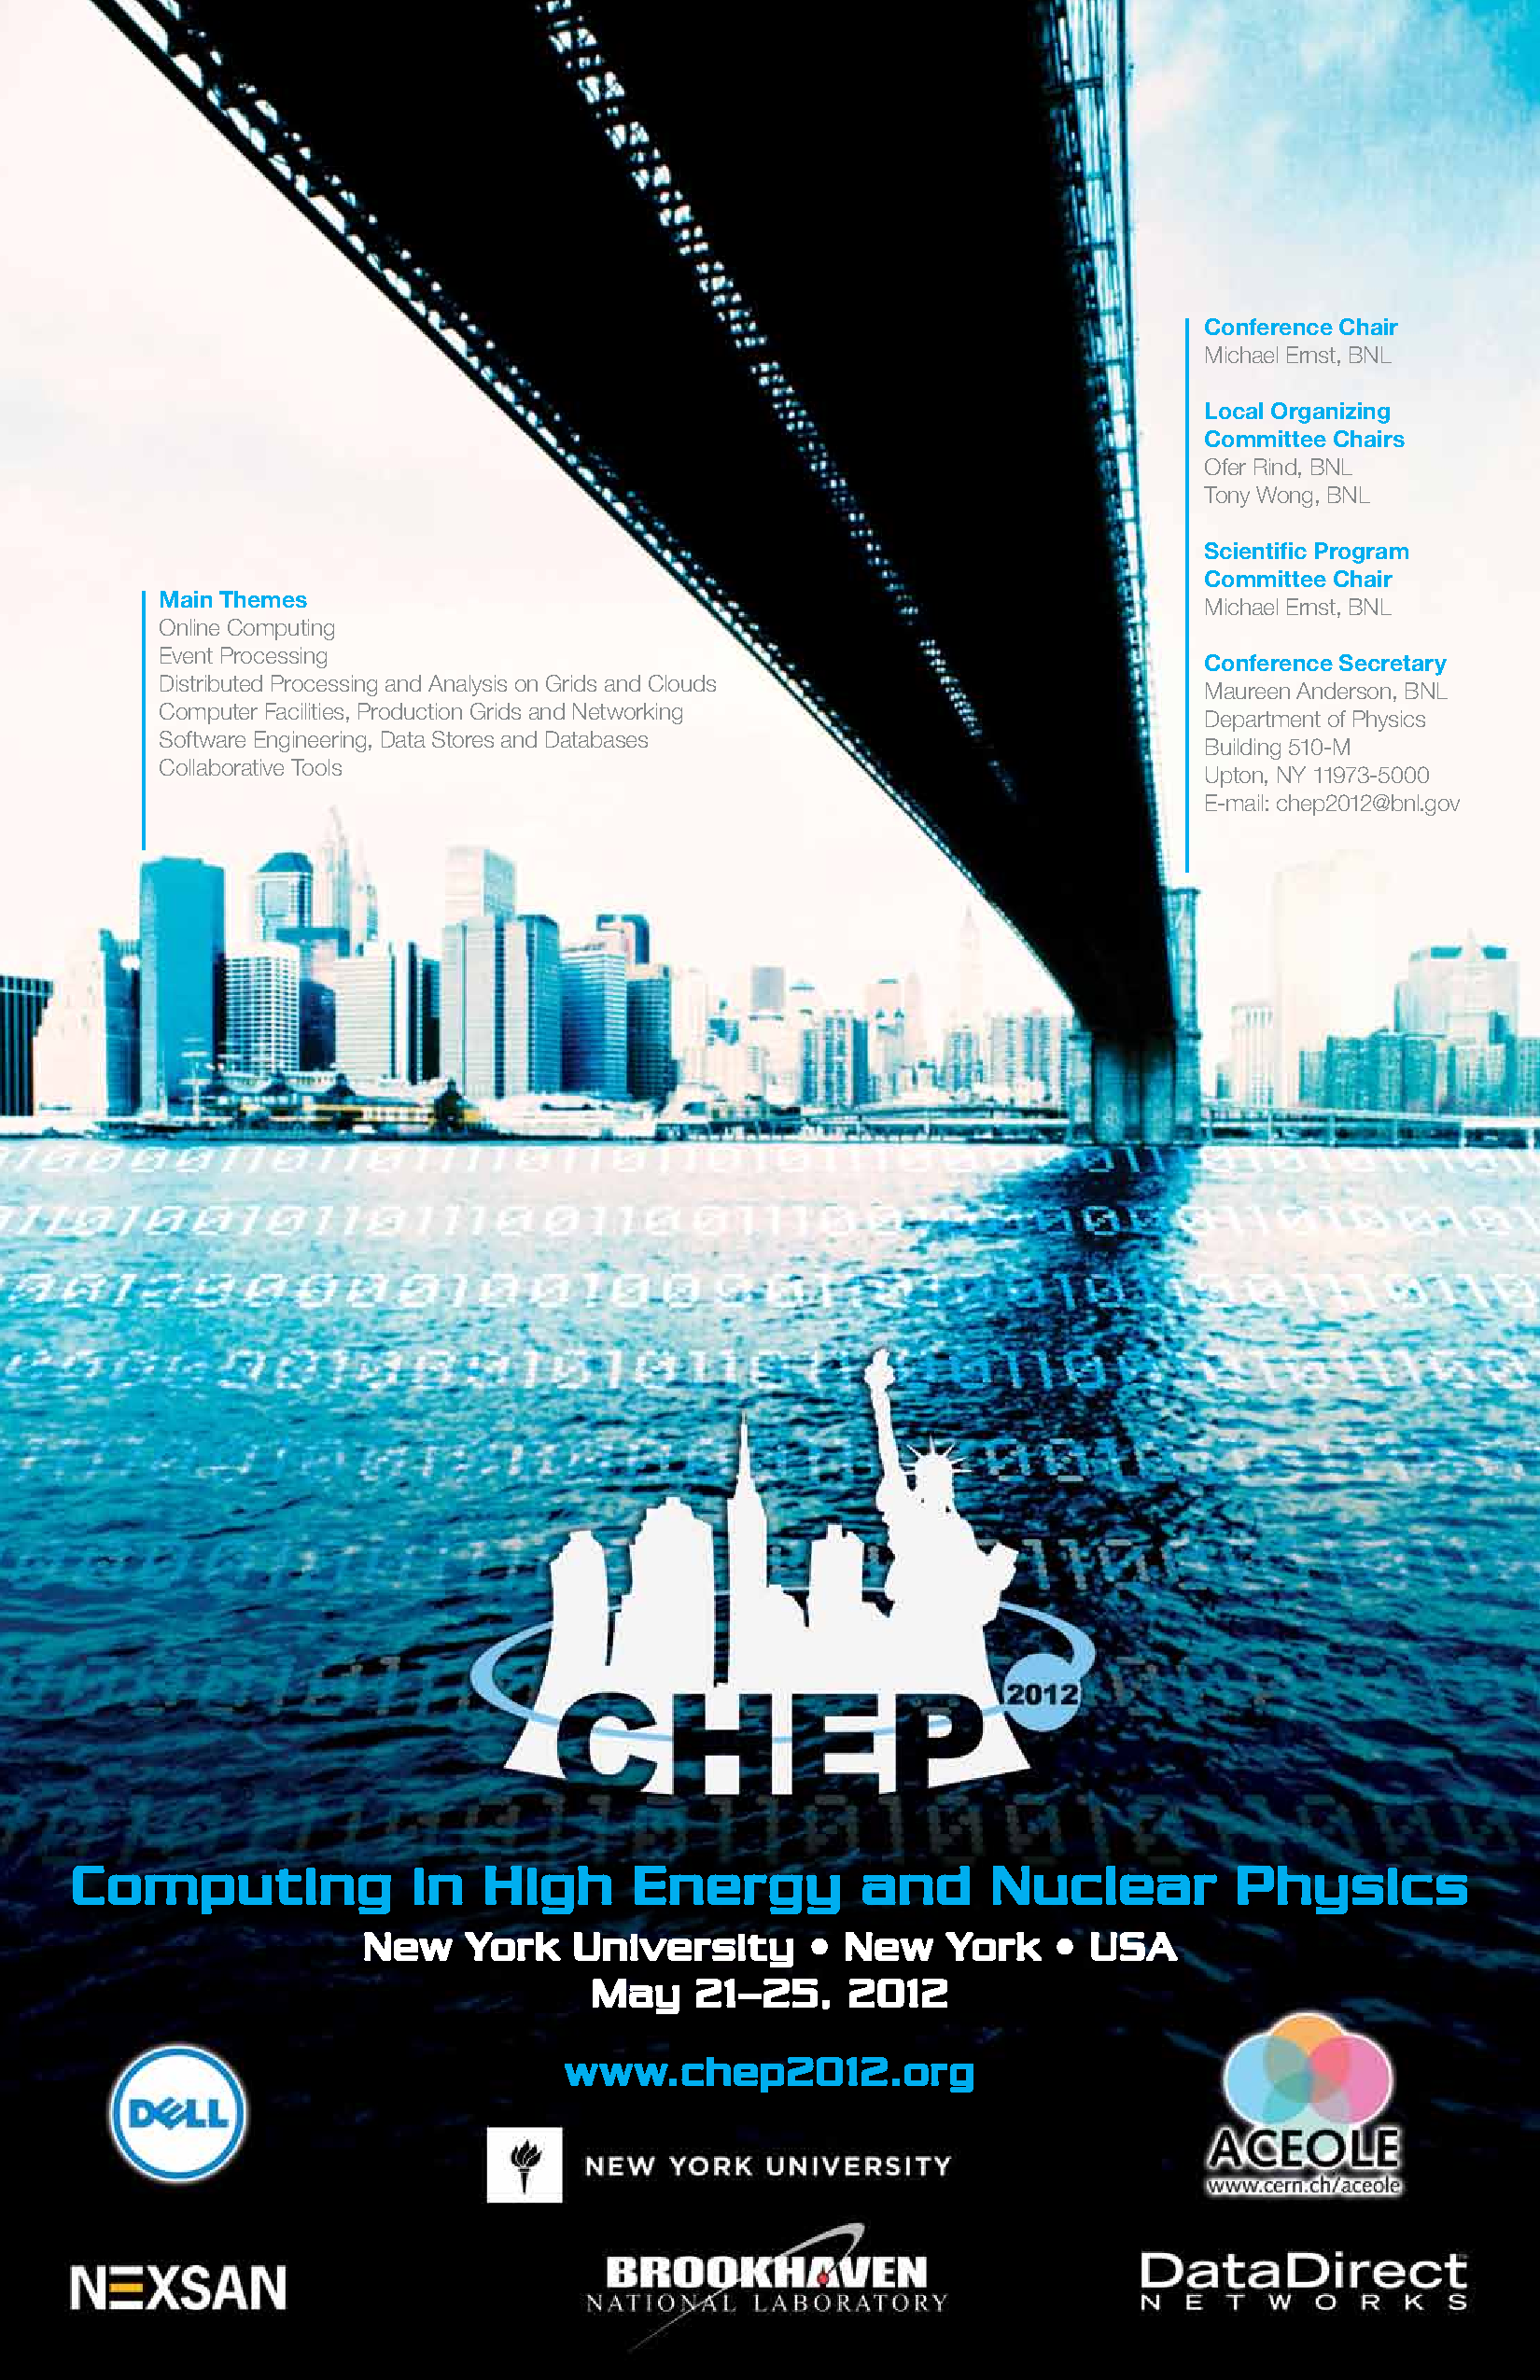
\includegraphics[height=6cm]{CHEP2012_poster.pdf}
\end{center}
\end{columns}
\end{frame}
\begin{frame}
\frametitle{Outline}
\tableofcontents
% You might wish to add the option [pausesections]
\end{frame}

\section{Content}
\begin{frame}
\frametitle{CHEP2012: what it was}
\begin{itemize}
  \item 7 plenary sessions
  \item 3 plenary summary sessions
  \item 6 parallel sessions
  \item 162 talks
  \item more than 200 posters (too many)
  \item 1 cocktail party
  \item 1 boat
\end{itemize}
I only present what was stricking to me
\end{frame}

\section{ROOT}
\begin{frame}
\frametitle{ROOT}
ROOT 6 planned for November:
\begin{itemize}
  \item CINT replaced by CLING (based on CLANG, how original\ldots)
  \item CLANG becomes the default compiler
  \item Use of OSX graphics libraries (quartz)
  \item ROOT on iOS/iPad, later Android
  {\tiny
  \url{https://indico.cern.ch/contributionDisplay.py?sessionId=0&contribId=587&confId=149557}}
  \item javascript library for online browsing of plots 
  {\tiny
  \url{https://indico.cern.ch/contributionDisplay.py?sessionId=6&contribId=170&confId=149557}}
\end{itemize}
I was disappointed by ROOT: too much focus on OSX and iOS, when I went to ask
for the completion of TH2Poly (used in Lumi analysis) they sent me from one guy to
the next.
\end{frame}

\begin{frame}
\frametitle{Additions to ROOT/G4}
New software library of geometrical primitives for modelling of solids used in
Monte Carlo detector simulations: Much faster than existing libs.\\
{\tiny
\url{https://indico.cern.ch/contributionDisplay.py?sessionId=6&contribId=401&confId=149557}}
\end{frame}

\section{EVO}
\begin{frame}
\frametitle{EVO $\to$ Seevogh}
EVO has no more funding at the end of the year $\to$ becomes a commercial
product
\begin{itemize}
  \item Used talk on review of VC in HEP for self promotion
  \item No mention of price
  \item What they offer does not match what others do, so why go there?
\end{itemize}
{\tiny
\url{https://indico.cern.ch/contributionDisplay.py?sessionId=0&contribId=608&confId=149557<}}
\end{frame}
\section{Software Engineering}
\begin{frame}
\frametitle{Software Engineering}
``If we knew what we were doing we would not call it research''\\

~\\

How to use the methods used in industry, and how do they use ours?\\
{\tiny
\url{https://indico.cern.ch/contributionDisplay.py?sessionId=0&contribId=589&confId=149557}}
\end{frame}

\section{The rest}
\begin{frame}
\frametitle{The rest}
\begin{itemize}
  \item PROOF on demand (PoD): Brilliant talk, very exciting, should give it a
  shot.\\ {\tiny
  \url{https://indico.cern.ch/contributionDisplay.py?sessionId=4&contribId=22&confId=149557}}
  \item Electronic Collaboration Logbook (ECL): very complete tool. No idea
  where we can get it (or if it's opensource/free). Mail sent.\\
  {\tiny
  \url{https://indico.cern.ch/contributionDisplay.py?sessionId=7&contribId=531&confId=149557}}
  \item Data preservation in HEP: 1 plenary, a few posters, and a dedicated
  parallel session.\\
  {\tiny
  \url{https://indico.cern.ch/contributionDisplay.py?sessionId=0&contribId=607&confId=149557}}
\end{itemize}
\end{frame}

\section{Overall}
\begin{frame}
\frametitle{Overall}
\begin{itemize}
  \item Not so many common tools: people are keeping their babies
  \item Too many talks of application for iOS (even G4!!!!)
  \item CLOUD computing, GPU usage, parallel processing tend to become the norm
  \item ILC/CLIC do not exist for that community, even for the future on
  computing, the plenary talk does not mention it\\
  {\tiny
  \url{https://indico.cern.ch/contributionDisplay.py?sessionId=0&contribId=606&confId=149557}}
\end{itemize}
\end{frame}
\section{Conclusion}
\begin{frame}
\frametitle{Conclusion}
\begin{itemize}
  \item Very interesting conference
  \item Both exciting and frustrating talks
  \item Next CHEP October 2013, Amsterdam
\end{itemize}
Also: very lengthy discussions with Norman/Jeremy/Andrei for SiD DBD
\end{frame}

\begin{frame}
\begin{center}
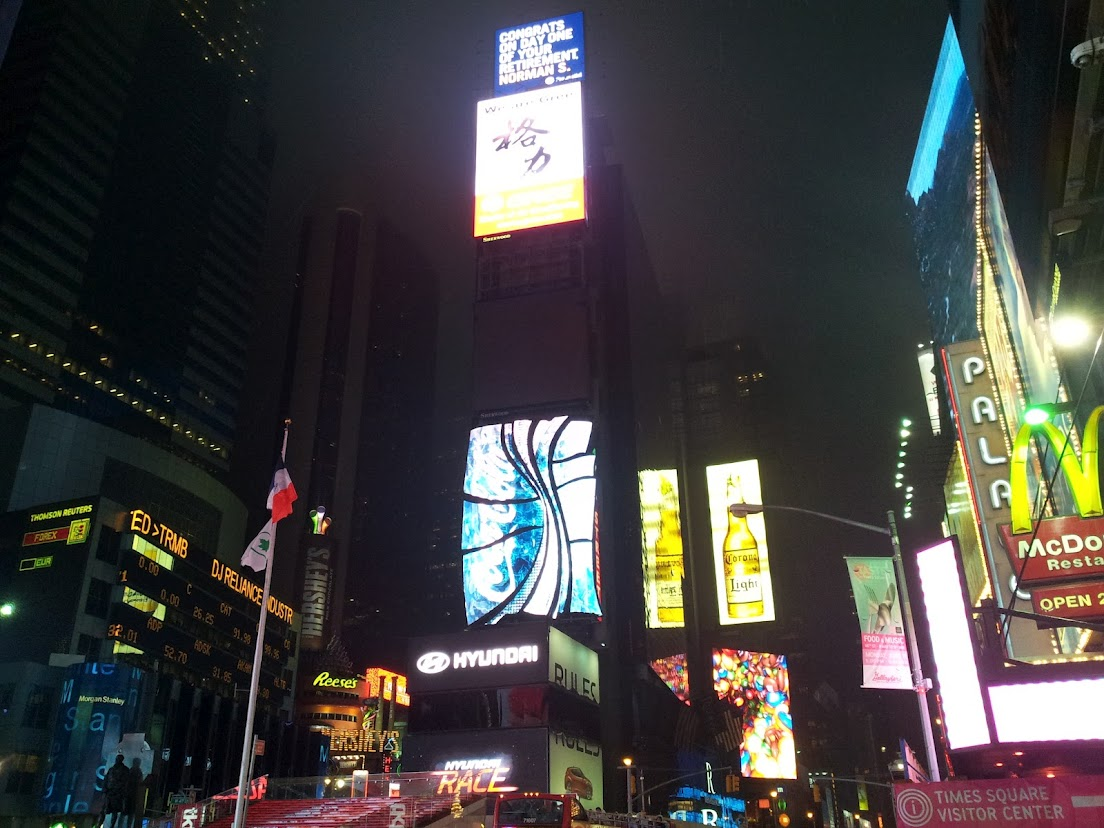
\includegraphics[width=8cm]{timesquare}
\end{center}
\end{frame}
\begin{frame}
\begin{center}
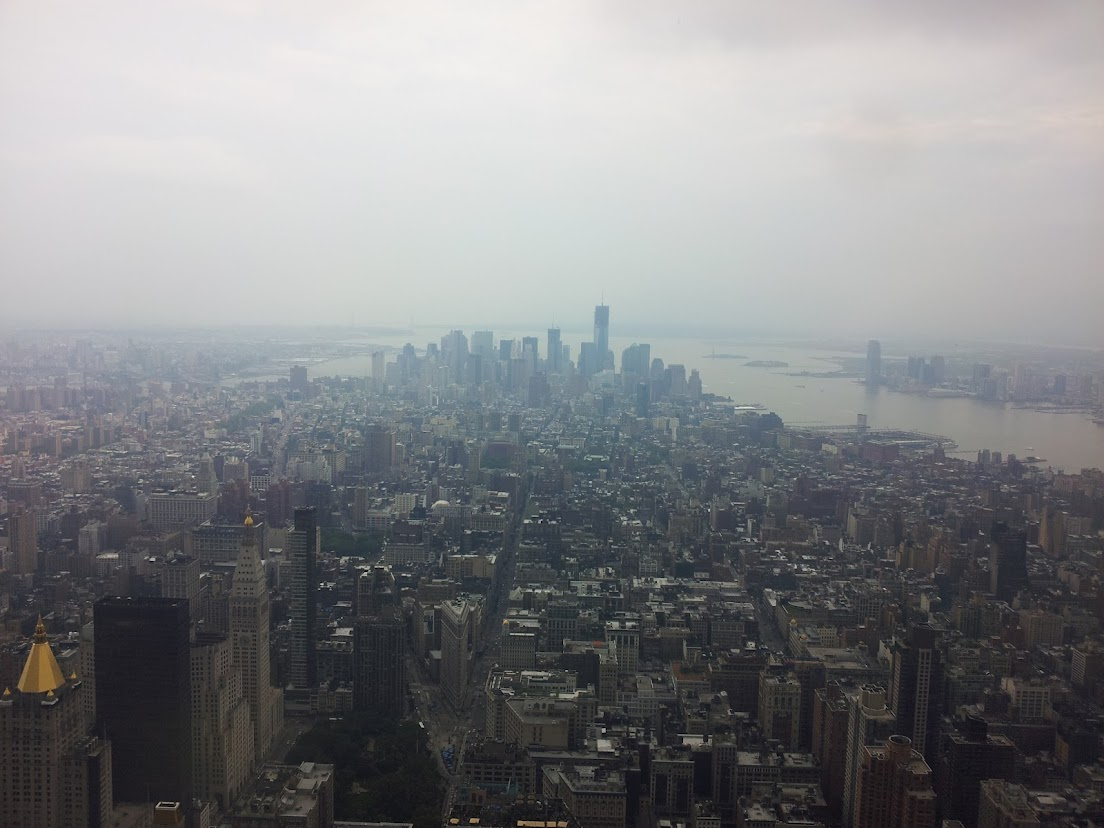
\includegraphics[width=8cm]{Empire}
\end{center}
\end{frame}
\begin{frame}
\begin{center}
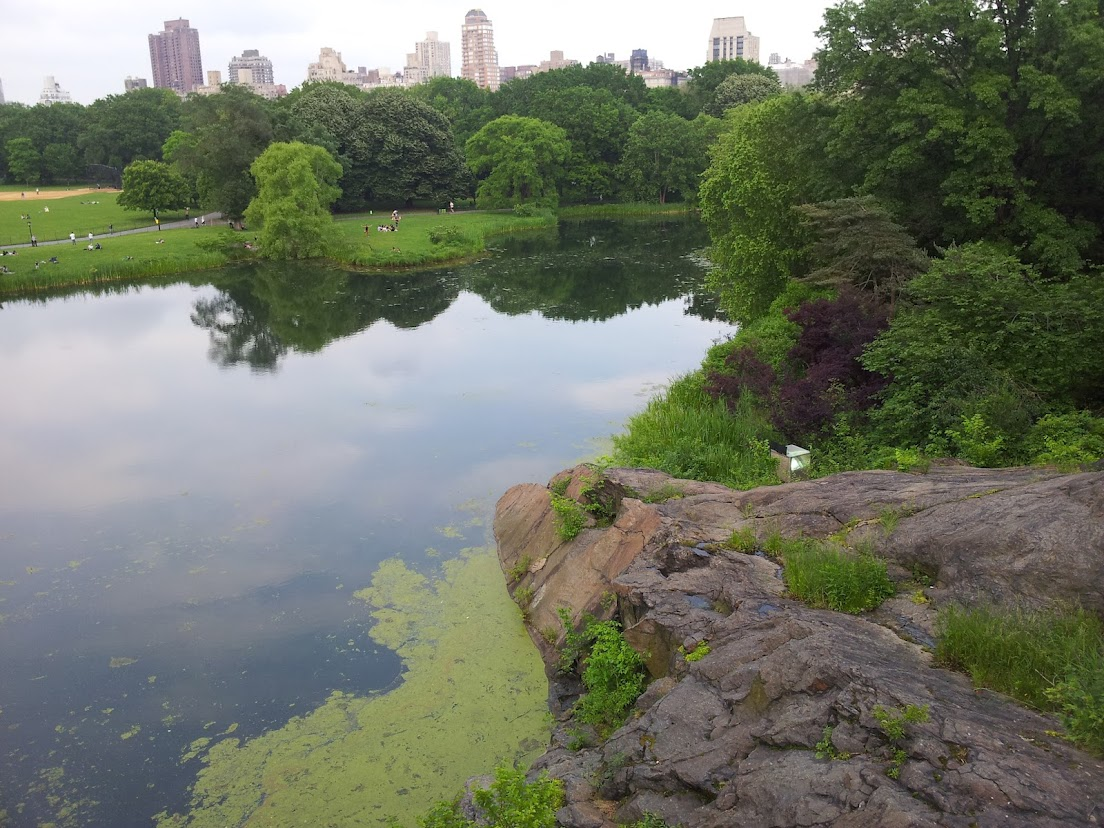
\includegraphics[width=8cm]{park}
\end{center}
\end{frame}
\begin{frame}
\begin{center}
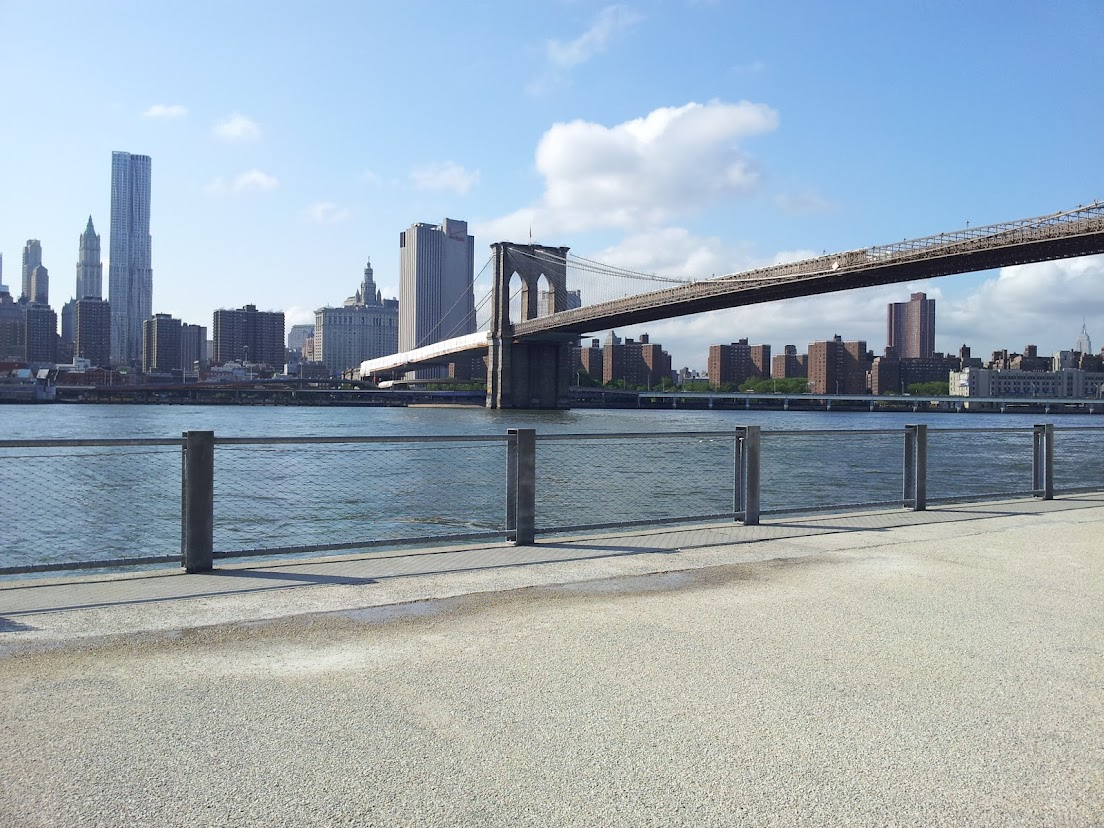
\includegraphics[width=8cm]{bridge}
\end{center}
\end{frame}
\begin{frame}
\begin{center}
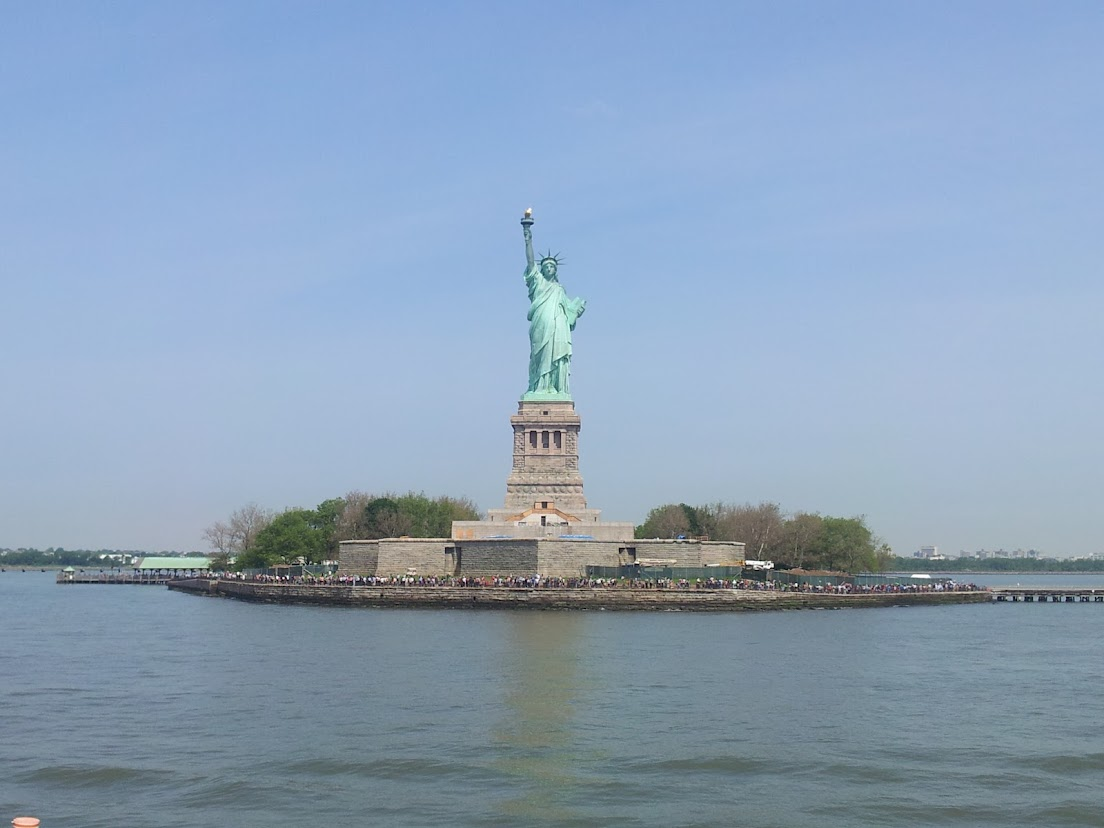
\includegraphics[width=8cm]{liberty}
\end{center}
\end{frame}
\end{document}